\documentclass[11pt]{article}
%\usepackage{amsfonts}
\usepackage{amsmath}
\usepackage{fancybox}%,times}
\usepackage{graphicx,psfrag,epsf}
%\usepackage{amsmath}
\usepackage{enumerate}
\usepackage{graphicx,psfrag}
\usepackage{multirow}
\usepackage{epsfig}
%\usepackage{rotating}
\usepackage{subfigure}
\usepackage{theorem}
\usepackage{natbib,psfrag}
\usepackage{tikz}
\usepackage{xcolor}
\usepackage{kotex}
\newcommand{\blind}{0}
\usepackage{graphicx}
\DeclareGraphicsExtensions{.pdf,.png,.jpg}

\addtolength{\oddsidemargin}{-.75in}%
\addtolength{\evensidemargin}{-.75in}%
\addtolength{\textwidth}{1.5in}%
\addtolength{\textheight}{1.3in}%
%\addtolength{\topmargin}{-.6in}%
\addtolength{\topmargin}{-.8in}%

%\theoremstyle{break}
\newtheorem{The}{Theorem}
\newtheorem{Def}{Definition}
\newtheorem{Pro}{Proposition}
\newtheorem{Lem}{Lemma}
\newtheorem{Cor}{Corollary}
\newtheorem{asp}{Assumption}


\renewcommand{\thefootnote}{\arabic{footnote}}
%\renewcommand{\thefootnote}{\alph{footnote}}
%\renewcommand{\thefootnote}{\roman{footnote}}
%\renewcommand{\thefootnote}{\fnsymbol{footnote}}

\begin{document}


%\bibliographystyle{natbib}

\newcommand{\Ito}{$It\hat{o}$'$s~Lemma$}

\newcommand\ind{\stackrel{\rm ind}{\sim}}
\newcommand\iid{\stackrel{\rm iid}{\sim}}
\renewcommand\c{\mathbf{c}}
\newcommand\y{\mathbf{y}}
\newcommand\z{\mathbf{z}}
\renewcommand\P{\mathbf{P}}
\newcommand\W{\mathbf{W}}
\newcommand\X{\mathbf{X}}
\newcommand\Y{\mathbf{Y}}
\newcommand\Z{\mathbf{Z}}
\newcommand\J{{\cal J}}
\newcommand\B{{\cal B}}
\newcommand\K{{\cal K}}
\newcommand\N{{\rm N}}
\newcommand\bs{\boldsymbol}
\newcommand\bth{\bs\theta}
\newcommand\bbe{\bs\beta}
\renewcommand\*{^\star}

\def\spacingset#1{\renewcommand{\baselinestretch}%
{#1}\small\normalsize} \spacingset{1}


%%%%%%%%%%%%%%%%%%%%%%%%%%%%%%%%%%%%%%%%%%%%%%%%%%%%%%%%%%%%%%%%%%%%%%%%%%%%%%

  \bigskip
  \bigskip
  \bigskip
  \begin{center}
    {\LARGE\bf October 8, 2018 }
  \end{center}
  \medskip

%\begin{abstract}
%\end{abstract}

%\noindent%
%{\it Key Words:}  AECM algorithm; Astrophysical data analysis;
%ECME algorithm; Incompatible Gibbs sampler; Marginal data
%augmentation; Multiple imputation; Spectral analysis

\spacingset{1.45}













\section{Gene network}
\label{sec:method}

 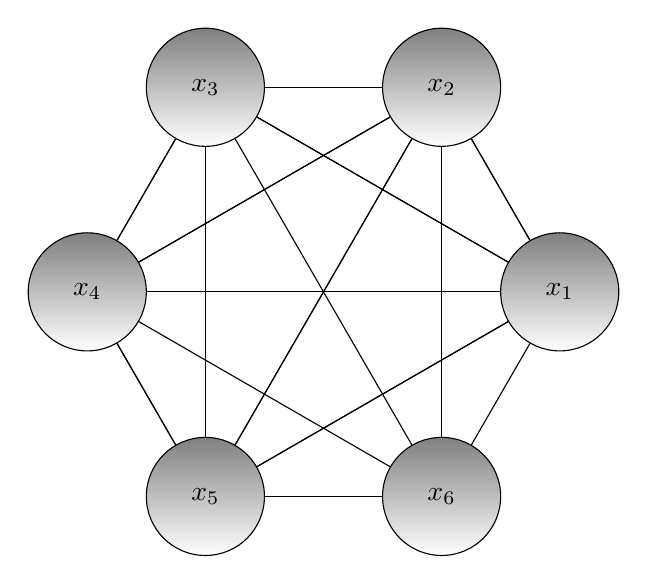
\begin{tikzpicture}
  \foreach \x /\alph/\name in {0/a/$x_{1}$, 60/b/$x_{2}$, 120/c/$x_{3}$, 180/d/$x_{4}$, 240/e/$x_{5}$, 300/f/$x_{6}$}{
  \node[circle, fill=green,minimum width=15mm,draw,shading=axis] (\alph) at (\x:3cm) {\name}; }

  \foreach \alpha in {a,b,c,d,e,f}%
  {%
  \foreach \alphb in {a,b,c,d,e}%
  {%
   \draw (\alpha) -- (\alphb);%
  }}

 \end{tikzpicture}

\begin{itemize}
\item Each node corresponds to a gene
\item Each edge corresponds to a pair of genes which are ‘co-expressed’
\end{itemize}
‘co-expressed’ meaning that their expression levels are highly correlated. The weights represent the strength of the connection between two genes.

True correlation between gene m,n $\rho_{mn}$ and correlation by observed data is $r_{mn} = corr(x_{m},x_{n})$
by Fisher's z-transformation $w_{mn} = arctanh(r_{mn})$ aproximately normal distribution .
  \begin{align}
    w_{mn} &\sim N(arctanh(\rho_{mn}), \frac{1}{N-3})
  \end{align}
Let E =\{$e_{mn}$\} be a set of true edges in the network.

The number of Gene $G$ is larger and that most paris ar not co-expressed, and the number of possible edge $K=G(G-1)/2$ is very larger than the number of true edges in the network $|E|$

So in this gene network model we have some assumption
\begin{itemize}
\item This graphical model is undirected model because each node means correlation
\item The network can be cycle??
\item The network is sparse ( $|E| << K$ )
\item The weight $w_{mn}$ follows $L_{2}N$ model 
\end{itemize}
 $L_{2}N$ model is a three component mixture model. First the 'null' component follow normal distribution with mean 0, which means majority of correlation between genes are 0. And the 'not null' components which mean strong positive/negative correlation follow log-normal distribution each.

\begin{figure}[htbp]
\begin{center}
    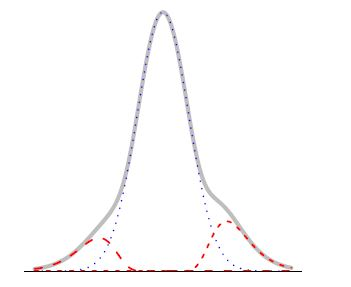
\includegraphics[scale=1.2]{fig_jpg}
    \caption{$L_{2}N$ model} \label{fig:label}
\end{center}
\end{figure}
  \begin{align}
    w_{mn}|e_{mn}\notin E &\sim N(0,\sigma^2)                 \\
    w_{mn}|[w_{mn}>0,e_{mn}\in E] &\sim LogNormal(\theta_{1},\kappa_{1}^2) 	\\
    - w_{mn}|[w_{mn}<0,e_{mn}\in E] &\sim LogNormal(\theta_{2},\kappa_{2}^2)
  \end{align}

$\sigma^2 = 1/(N-3) + \sigma_{0}^2$ ,where $1/(N-3)$ from Fisher's z-transformation and $\sigma_{0}^2$ from random effect model.
Let $C_{0}, C_{1}, C_{2}$ means the distribution in the mixture model $C_{0}$ the null component, $C_{1}, C_{2}$ the 2 not null components.

  \begin{align}
    Pr(e_{mn} \in C_{j}|w_{mn}) & = \frac{P_{j}f_{j}(w_{mn})}{P_{0}f_{0}(w_{mn})+P_{1}f_{1}(w_{mn})P_{2}f_{2}(w_{mn})}
  \end{align}

$\textbf{b}_{mn}$ =$(b_{mn0},b_{mn1},b_{mn2})$ means the indicator vector $b_{mnj} = 0$  when the $Pr(e_{mn} \in C_{j}|w_{mn}) $ has the highest probablity and 0 for the other two. Make adjacency $G \times G$ matrix $\textbf{A}$, where $\textbf{A}_{mn} = 1- b_{mn0}$ , 
\section{Hill Climbing}
A bayesian network, DAG \
\end{document}
